\cardfrontfoot{Kapitel 15}

\begin{flashcard}[Egenskab]{Hvordan fremstår grundstofferne i 5. hovedgruppe ved SATP?}
Nitrogen er en farveløs gas. Fosfor er en hvis voks-agtig substans. De resterende er skrøblige metaller.
\end{flashcard}

\begin{flashcard}[Teori]{Angiv de specier der har tendens til at disproportionere i sur opløsning\\
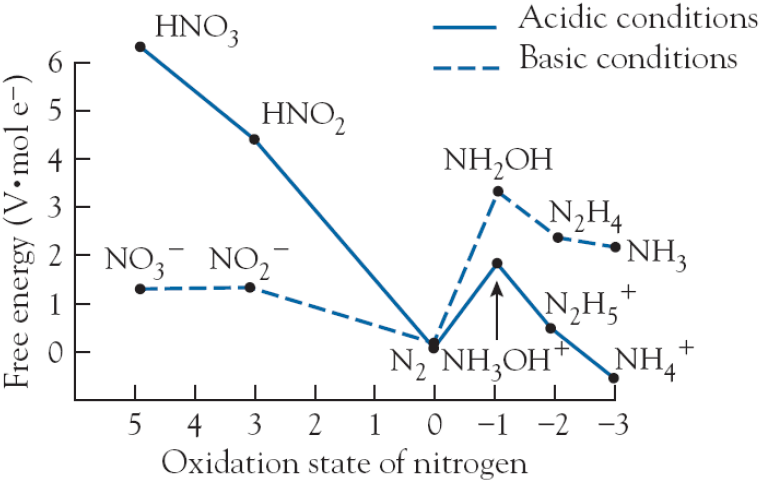
\includegraphics[width=0.55\textwidth]{figures/k15s368FrostDiagram.png}
}
\ce{HNO2} samt \ce{NH3OH+}
\end{flashcard}

\begin{flashcard}[Fremstilling]{Angiv hvordan ammoniak kan fremstilles i laboratoriet}
\ce{NH4Cl + NaOH -> NH3(g) + NaCl}
\end{flashcard}

\begin{flashcard}[Fremstilling]{Opskriv hvordan ammoniak fremstilles industrielt}
\ce{CH4 + H2O -> CO + 3H2}\\
\ce{ZnO + H2S -> ZnS + 2H2O}\\
\ce{Ch4 + $\frac{1}{2}$O2 + 2N2 -> CO + 2H2 + 2N2}\\
\ce{CO + H2O <=> CO + H2}\\
\ce{CO2 + K2CO3 + H2O <=> 2KHCO3}\\
\ce{ N_{2} + 3H_{2} <=> 2NH_{3}}\\ \vspace{7pt}
ved et tryk på 100-1000 atm og en temperatur på 400-500$\,^{\circ}{\rm C}$
\end{flashcard}

\begin{flashcard}[Egenskab]{Reagerer hydrazin alkalisk eller neutralt?}
Alkalisk\\ \vspace{7pt}
\ce{N2H4 + H3O+ -> N2H5+ + H2O}
\end{flashcard}

\begin{flashcard}[Egenskab]{Angiv hvordan hydrazin kan anvendes som reduktionsmiddel}
\ce{N2H4 + 2I2 -> 4HI + N2}\\ \vspace{7pt}
\ce{N2H4 + 2Cu^{2+} -> 2Cu + N2 + 4H+}
\end{flashcard}

\begin{flashcard}[Struktur]{Tegn hydrazin}
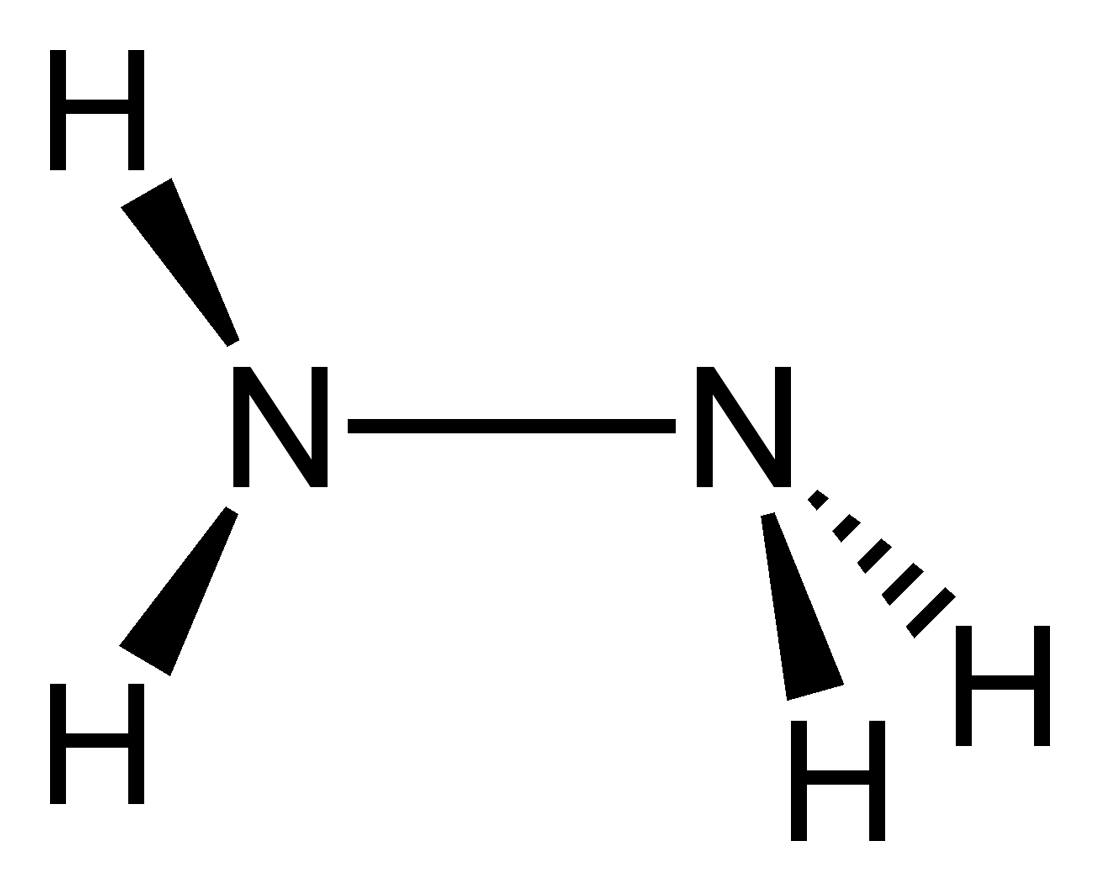
\includegraphics[width=0.55\textwidth]{figures/Hydrazin.png}
\end{flashcard}

\begin{flashcard}[Reaktion]{Angiv hvordan hydrogenazid dekomponerer}
\ce{2HN3 -> H2 + 3N2}
\end{flashcard}

\begin{flashcard}[Anvendelse]{Forklar hvordan en airbag virker ved hjælp af reaktionsligninger}
\ce{2NaN3 ->[\text{$\Delta$}] 2Na(l) + 3N2}\\
\ce{10Na(l) + 2KNO3 -> K2O + 5Na2O + N2}\\
\ce{2K2O + SiO2 -> K4SiO4}\\
\ce{2Na2O + SiO2 -> Na4SiO4}
\end{flashcard}

\begin{flashcard}[Reaktion]{Angiv hvordan følgende forbindelser dekomponerer ved opvarmning\\
\ce{NH4NO2}, \ce{NH4NO3} samt \ce{(NH4)2Cr2O7}
}
\ce{NH4NO2 ->[\text{$\Delta$}] N2 + 2H2O}\\ \vspace{7pt}
\ce{NH4NO3 ->[\text{$\Delta$}] N2O + 2H2O}\\ \vspace{7pt}
\ce{(NH4)2Cr2O7 ->[\text{$\Delta$}] N2 + Cr2O3 + 4H2O}
\end{flashcard}

\begin{flashcard}[Reaktion]{Angiv en metode til at producere lattergas}
\ce{NH4NO3 ->[\ce{H+}] N2O + 2H2O}
\end{flashcard}

\begin{flashcard}[Reaktion]{Angiv en metode til at producere nitrogenmonoxid}
\ce{3Cu + 8HNO3 -> 3Cu(NO3)2 + 4H2O + 2NO}
\end{flashcard}

\begin{flashcard}[Reaktion]{Angiv en metode til at producere \ce{N2O3}}
\ce{NO + NO2 -> N2O3(l)}
\end{flashcard}

\begin{flashcard}[Reaktion]{Angiv reaktionen mellem \ce{N2O3} og vand}
\ce{N2O3 + H2O -> 2HNO2}
\end{flashcard}

\begin{flashcard}[Struktur]{Tegn dinitrogentrioxid}
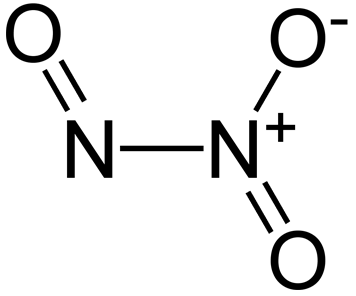
\includegraphics[width=0.55\textwidth]{figures/Dinitrogentrioxid.png}
\end{flashcard}

\begin{flashcard}[Reaktion]{Angiv to metoder til at producere nitrogendioxid}
\ce{Cu + 4HNO3 -> Cu(NO3)2 + 2H2O + 2NO2}\\ \vspace{7pt}
\ce{Cu(NO3)2 ->[\text{$\Delta$}] CuO + 2NO2 + $\frac{1}{2}$O2}
\end{flashcard}

\begin{flashcard}[Reaktion]{Angiv reaktionen mellem nitrogendioxid og vand}
\ce{2NO2 + H2O <=> HNO3 + HNO2}
\end{flashcard}

\begin{flashcard}[Struktur]{Tegn nitrogendioxid}
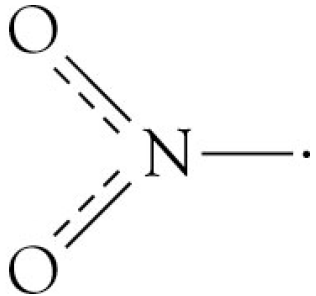
\includegraphics[width=0.3\textwidth]{figures/k15s383Nitrogendioxid.png}
\end{flashcard}

\begin{flashcard}[Struktur]{Tegn dinitrogentetroxid}
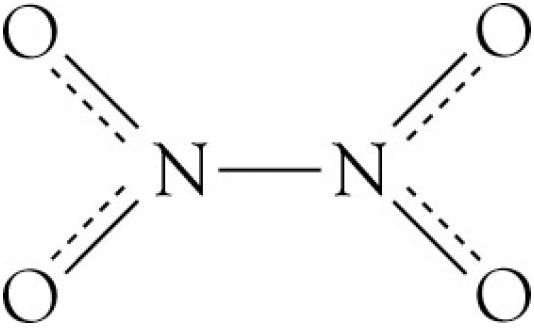
\includegraphics[width=0.5\textwidth]{figures/k15s383Dinitrogentetroxid.png}
\end{flashcard}

\begin{flashcard}[Struktur]{Tegn dinitrogenpentoxid}
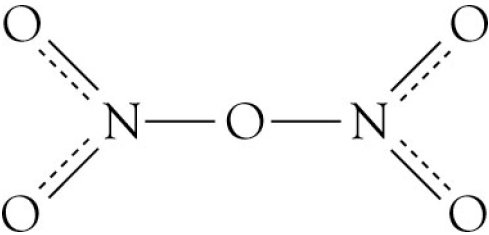
\includegraphics[width=0.5\textwidth]{figures/k15s383Dinitrogenpentoxid.png}
\end{flashcard}

\begin{flashcard}[Struktur]{Tegn nitrat}
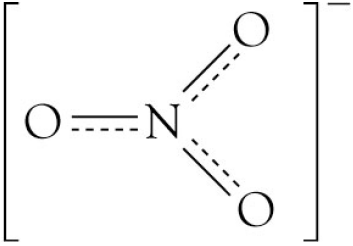
\includegraphics[width=0.5\textwidth]{figures/k15s383Nitrat.png}
\end{flashcard}

\begin{flashcard}[Struktur]{Tegn nitrit}
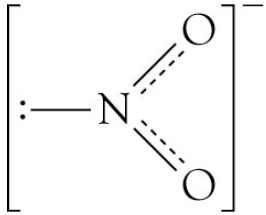
\includegraphics[width=0.5\textwidth]{figures/k15s385Nitrit.png}
\end{flashcard}

\begin{flashcard}[Fremstilling]{Angiv med reaktionsligning hvordan man kan fremstille salpetersyrling i laboratoriet}
\ce{Ba(NO2)2 + H2SO4 -> BaSO4(s) + 2HNO2}
\end{flashcard}

\begin{flashcard}[Reaktion]{Angiv med reaktionsligning hvordan salpetersyrling disproportionerer}
\begin{align*}
\ce{3H\OX{d,\ox{+3,\ce{N}}}O2 -> H\OX{oe1,\ox{5,\ce{N}}}O3 + 2\OX{re1,\ox{+2,\ce{N}}}O}
\redox(d,oe1){\small oxidation}
\redox(d,re1)[][-1]{\small reduktion}
\end{align*}\\ \vspace{15pt}
(\ce{2NO + O2 -> 2NO2})
\end{flashcard}

\begin{flashcard}[Fremstilling]{Opskriv hvordan man producerer salpetersyre industrielt via. Ostwald-processen}
\ce{4NH3 + 5O2 -> 4NO + 6H2O}\\
\ce{2NO + O2 -> 2NO2}\\
\ce{3NO2 + H2O -> 2HNO3 + NO}
\end{flashcard}

\begin{flashcard}[Anvendelse]{Angiv den eksoterme reaktion der finder sted i en cold pack}
\ce{NH4NO3(s) -> NH4+ + NO3-}
\end{flashcard}

\begin{flashcard}[Struktur]{Tegn strukturen af hvid henholdsvis rød fosfor}
Hvid:\\
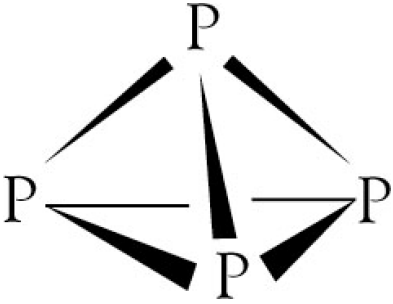
\includegraphics[width=0.2\textwidth]{figures/k15s390HvidP.png}\\
Rød:\\
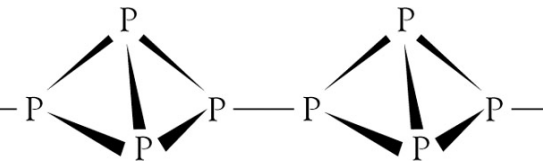
\includegraphics[width=0.6\textwidth]{figures/k15s390RodP.png}
\end{flashcard}

\begin{flashcard}[Reaktion]{Hvad sker der med hvid fosfor der udsættes for UV lys?}
Det omdannes til dens allotrop, rød fosfor
\end{flashcard}

\begin{flashcard}[Reaktion]{Hvorfor skal hvid fosfor opbevares under vand?}
Fordi det reagerer med atmosfærens oxygen\\
\ce{P4 + 5O2 -> P4O10}
\end{flashcard}

\begin{flashcard}[Fremstilling]{Hvordan udvindes fosfor industrielt?}
\ce{2Ca3(PO4)2 + 10CO ->[\text{$\Delta$}] 6CaO + 10CO2 + P4(g)}\\
\ce{CO2 + C -> 2CO} \\
\ce{CaO + SiO2 ->[\text{$\Delta$}] CaSiO3(l)}\\ \vspace{7pt}
Reaktionerne foregår ved $\rm 1500\,^{\circ}{\rm C}$.
\end{flashcard}

\begin{flashcard}[Fremstilling]{Hvordan fremstilles phosphin?}
\ce{Ca3P2 + 6H2O(s) -> 2PH3 + 3Ca(OH)2}
\end{flashcard}

\begin{flashcard}[Reaktion]{Opskriv reaktionerne hvorved de to oxider af fosfor dannes}
\ce{P4 + 3O2 -> P4O6}\\ \vspace{7pt}
\ce{P4 + 5O2 -> P4O10}
\end{flashcard}

\begin{flashcard}[Struktur]{Tegn strukturen af \ce{P4O6}}
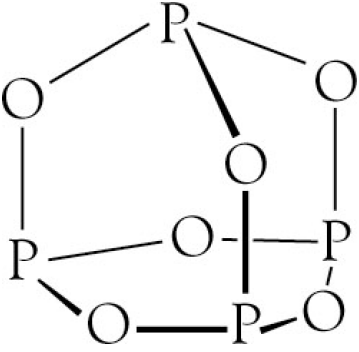
\includegraphics[width=0.4\textwidth]{figures/k15s393P4O6.png}
\end{flashcard}

\begin{flashcard}[Struktur]{Tegn strukturen af \ce{P4O10}}
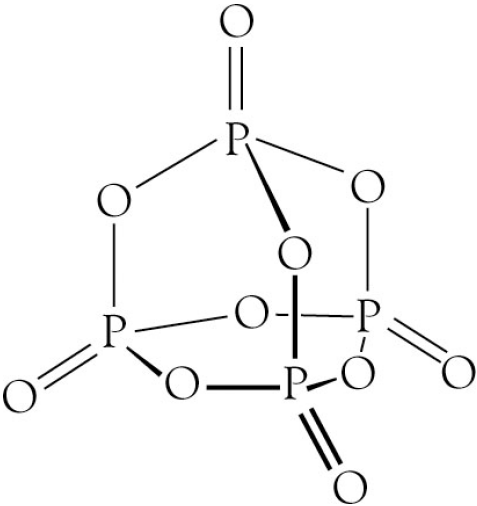
\includegraphics[width=0.4\textwidth]{figures/k15s394P4O10.png}
\end{flashcard}

\begin{flashcard}[Reaktion]{Angiv reaktionen mellem \ce{P4O10} og vand}
\ce{P4O10 + 6H2O + 4H3PO4}
\end{flashcard}

\begin{flashcard}[Reaktion]{Opskriv reaktionligninger for hvordan man danner de to chlorider af fosfor}
\ce{P4 + 6Cl2 -> 4PCl3}\\ \vspace{7pt}
\ce{P4 + 10Cl2 -> 4PCl5}
\end{flashcard}

\begin{flashcard}[Reaktion]{Angiv phosphortrichlorids henholdsvis phosphorpentachlorids reaktion med vand}
\ce{PCl3 + H2O -> H3PO3 + 3HCl}\\ \vspace{7pt}
\ce{PCl5 + H2O -> POCl3 + 2HCl}\\
\ce{POCl3 + 3H2O -> H3PO4 + 3HCl}
\end{flashcard}

\begin{flashcard}[Fremstilling]{Angiv med reaktionsskema hvorledes \ce{POCl3} fremstilles}
\ce{2PCl3 + O2 -> 2POCl3}
\end{flashcard}

\begin{flashcard}[Struktur]{Tegn \ce{H3PO4}, \ce{H3PO3} samt \ce{H3PO2}}
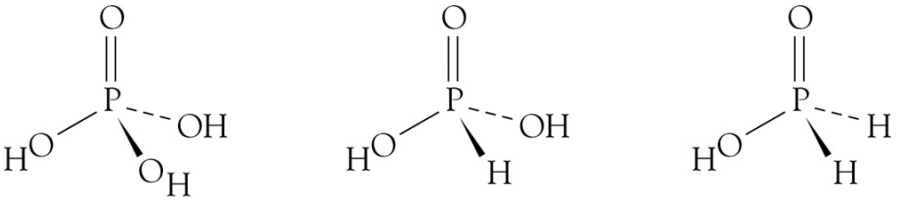
\includegraphics[width=0.9\textwidth]{figures/k15s395POxyAcids.png}
\end{flashcard}

\begin{flashcard}[Fremstilling]{Angiv hvordan fosforsyre fremstilles ved vådprocessen}
\ce{Ca3(PO4)2 + 3H2SO4 -> 3CaSO4(s) + 2H3PO4}
\end{flashcard}

\begin{flashcard}[Struktur]{Angiv strukturen af kondensationsproduktet der fås ved opvarmning af fosforsyre}
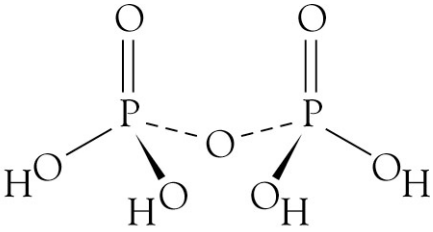
\includegraphics[width=0.6\textwidth]{figures/k15s396H4P2O7.png}
\end{flashcard}

\begin{flashcard}[Fremstilling]{Angiv med reaktionsskema hvordan calciumfosfat kan bearbejdes så det kan bruges som gødning}
\ce{Ca3(PO4)2(s) + 2H2SO4 -> Ca(H2PO4)2(s) + 2CaSO4(s)}
\end{flashcard}